\documentclass{article}

\usepackage{graphicx}
\usepackage{subcaption}


\title{Homework I: Iterative methods for sparse matrices}
\author{Lauren Devrieze}
\date{\today}

\begin{document}
	
	\maketitle
	
	\section*{Introduction}
	
	\section{Timing and memory of methods}
		
	In table \ref{tableTimings} the timings of all the methods combined with different preconditioners and the direct method are displayed. There are a few empty spots in the table when using matrix 2. For the preconditioners ILU(0) and ILU(1) all the methods can't be executed because the diagonal of the preconditioner multiplied with matrix 2 is zero.\\
	After looking at the longer timings, it can be concluded that generally GMRES(10) is the fastest method followed by BiCGStab and GMRES(100) is the slowest. The smaller timings don't have a significant difference in them so it's difficult to conclude something from them. \\
	The timings for the direct method aren't so clear. For matrix 3 it is faster, but for matrix 4 and 5, it is a lot slower. \\
	
	%timings
	\begin{table}[h]
		\centering
		\begin{tabular}{|l|c|c|c|c|c|}
			\hline
							 & Matrix 1 & Matrix 2 & Matrix 3 & Matrix 4 & Matrix 5 \\\hline \hline 
			BiCGStab (ILU(0)) & 0.040769 & 		& 62.3667 & 235.744 & 0.34591 \\ \hline
			BiCGStab (ILU(1)) & 2.53761 & 	     & 97.9519 & 418.621 & 0.954309 \\ \hline
			BiCGStab (ARMS)  & 0.012949 & 0.229775 & 48.2617 & 257.314 & 3.05756 \\ \hline \hline
			GMRES(10) (ILU(0)) &  0.04849 & 	 & 37.008 & 129.211 & 0.380574  \\ \hline
			GMRES(10) (ILU(1)) & 2.3546 & 	    & 58.8101 & 242.496 & 0.952507 \\ \hline
			GMRES(10) (ARMS) & 0.20596 & 0.2452 & 28.3702 & 170.48 & 3.1586 \\ \hline \hline
			GMRES(100) (ILU(0)) & 0.112047 &    & 81.9552 & 398.752 & 0.341786 \\ \hline
			GMRES(100) (ILU(1)) & 2.43374 &     & 95.0938 & 464.788 & 0.974389 \\ \hline
			GMRES(100) (ARMS) & 0.014858 & 0.013013 & 127.325 & 368.297 & 3.30781 \\ \hline \hline
			Direct method & 0.021279 & 0.022208 & 20.4651 & 737.353  & 15.2156 \\ \hline
		\end{tabular}
		\caption{Table with the timings for different methods with preconditioners and the direct method, expressed in seconds.}
		\label{tableTimings}
	\end{table}
	
	The memoryFor the memory usage it is clear that it's more dependent on the type of preconditioner than the type of method that is used. 
	
	%Memory usage
	\begin{table}[h]
		\centering
		\begin{tabular}{|l|c|c|c|c|c|}
			\hline
				 & Matrix 3 & Matrix 4 \\ \hline 
			BiCGStab (ILU(0)) & 2.8 & 10.2  \\ \hline
			BiCGStab (ILU(1)) & 3.7 & 15.5  \\ \hline
			BiCGStab (ARMS)  & 4 & 14.4 \\ \hline
			GMRES(10) (ILU(0)) &  2.8 & 10.5 \\ \hline
			GMRES(10) (ILU(1)) & 3.8 & 15.8 \\ \hline
			GMRES(10) (ARMS) & 4 & 14.4 \\ \hline
			GMRES(100) (ILU(0)) & 3.9 & 16.1 \\ \hline
			GMRES(100) (ILU(1)) & 4.9 & 21.3 \\ \hline
			GMRES(100) (ARMS) & 5.1 & 20.6 \\ \hline
		\end{tabular}
		\caption{Table with the memory usage for different methods and preconditioners, expressed in percent of the total memory.}
	\end{table}
	
	\begin{table}[h]
		\centering
		\begin{tabular}{|l|c|c|c|c|c|}
			\hline
						& Matrix 1 & Matrix 2 & Matrix 3 & Matrix 4 & Matrix 5 \\ \hline 
			without --ooc & 0.021279 & 0.022208 & 20.4651 &   & 15.2156 \\ \hline
			with --ooc & 0.113117 & 0.161896 & 23.5209 & 737.353 & 13.2442 \\ \hline
		\end{tabular}
		\caption{Table with the timings for the direct method, expressed in seconds.}
	\end{table}
	
	\begin{table}[h]
		\centering
		\begin{tabular}{|l|c|c|c|c|c|}
			\hline
			&  Matrix 3 & Matrix 4 & Matrix 5 \\ \hline 
			without --ooc & 11.6 &  & 5.3 \\ \hline
			with --ooc & 2.9 & 61.5 & 2.1 \\ \hline
		\end{tabular}
		\caption{Table with the memory usage for the direct method, expressed in percent of the total memory.}
	\end{table}
	
	
	\begin{figure}
		\centering
		\makebox[\linewidth][c]{%
		\begin{subfigure}[b]{0.65\textwidth}
			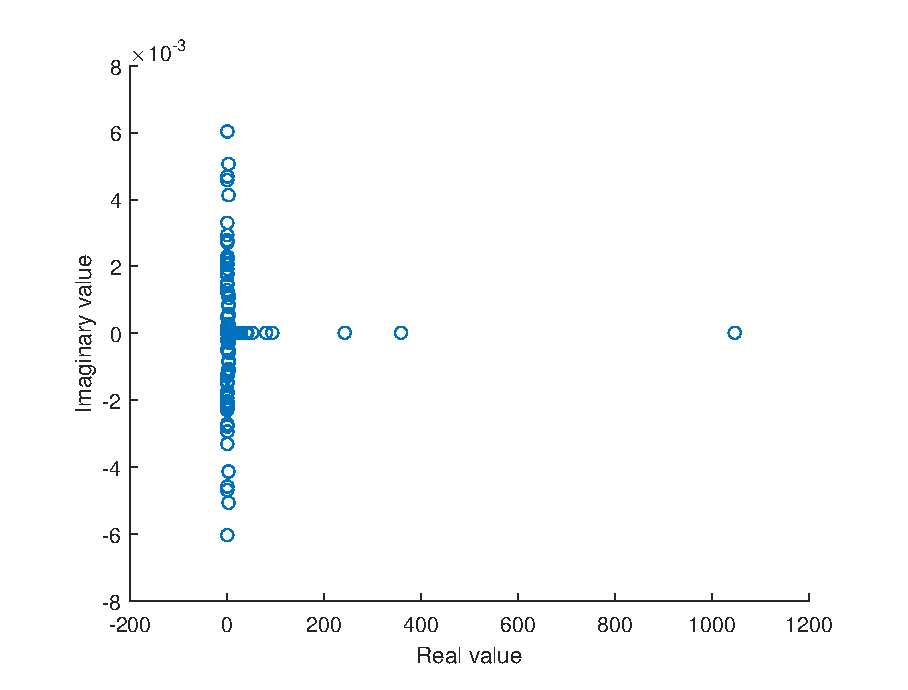
\includegraphics[width=\textwidth]{mat01_spectrum.eps}
			\caption{The spectrum of mat01.}
			\label{fig:mat01spectrum}
		\end{subfigure}
		~ 
		\begin{subfigure}[b]{0.65\textwidth}
			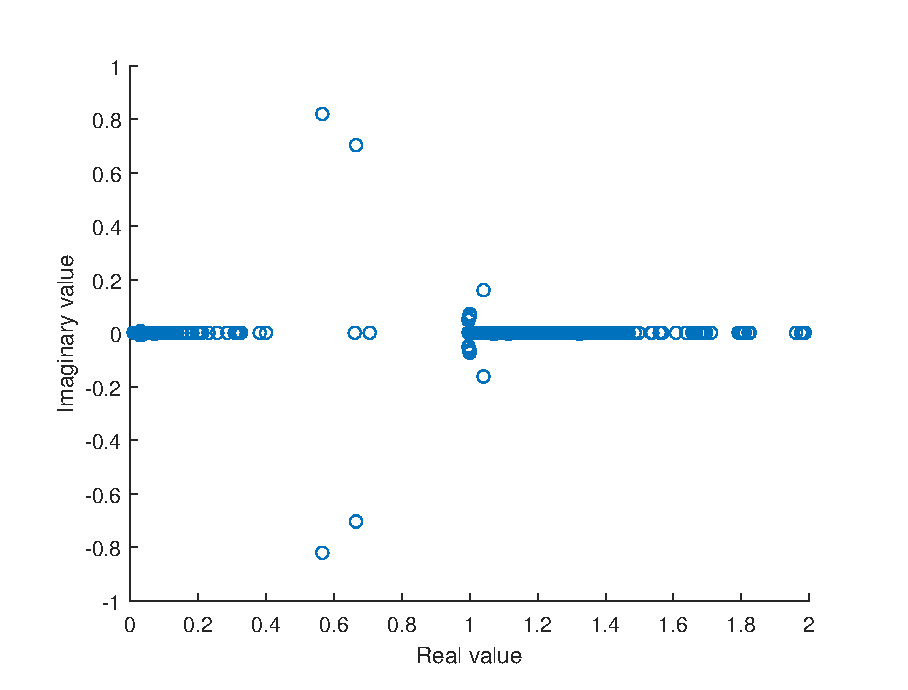
\includegraphics[width=\textwidth]{ILUK0_mat01_spec.eps}
			\caption{The spectrum of the preconditioner multiplied with mat01 in which the preconditioner ILU(0) is used.}
			\label{fig:ILUK0mat01spec}
		\end{subfigure}
		}	

		\makebox[\linewidth][c]{%
		\begin{subfigure}[b]{0.65\textwidth}
			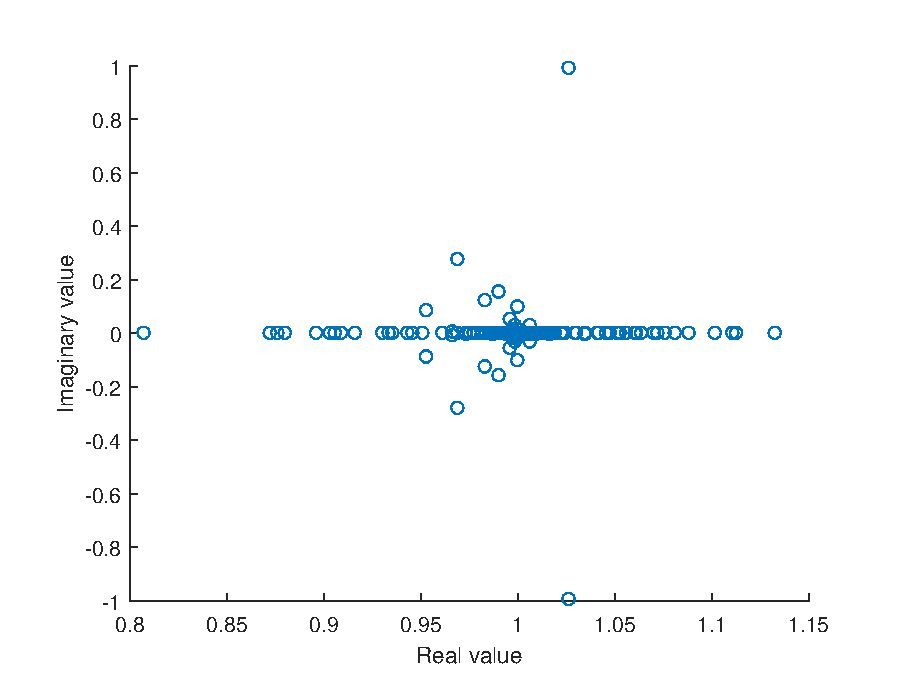
\includegraphics[width=\textwidth]{ILUK1_mat01_spec.eps}
			\caption{The spectrum of the preconditioner multiplied with mat01 in which the preconditioner ILU(1) is used.}
			\label{fig:ILUK1mat01spec}
		\end{subfigure}
		\begin{subfigure}[b]{0.65\textwidth}
			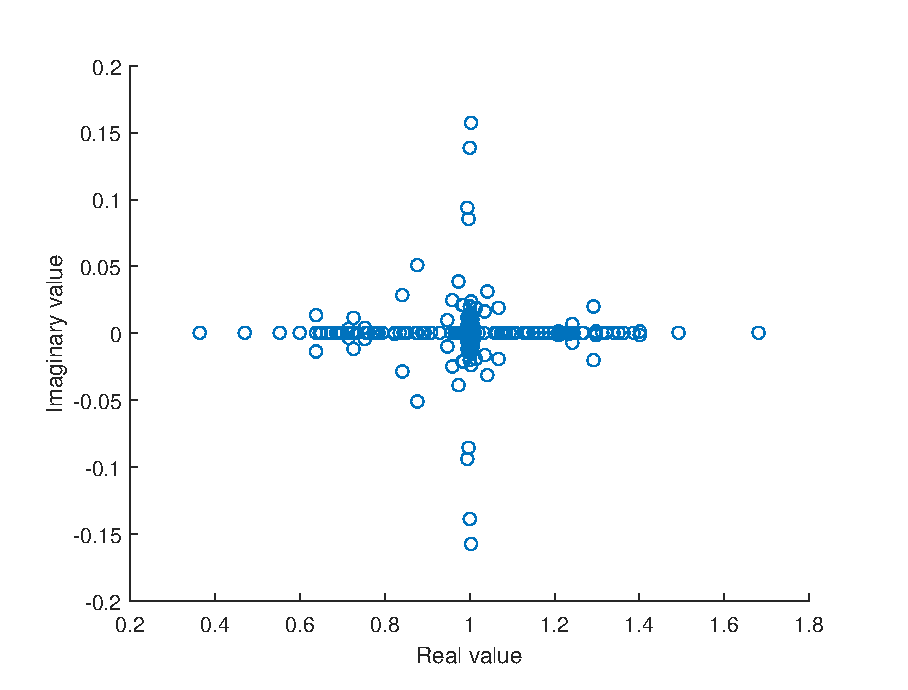
\includegraphics[width=\textwidth]{ARMS11_mat01_spec.eps}
			\caption{The spectrum of the preconditioner multiplied with mat01 in which the preconditioner ARMS is used with value k=1 and ARMS\_levels=1.}
			\label{fig:ARMS11mat01spec}
		\end{subfigure}
		}
		\caption{Spectra of mat01 with different preconditioners.}\label{fig:spectramat01}
	\end{figure}
	
	\begin{figure}
		\centering
		\makebox[\linewidth][c]{%
			\begin{subfigure}[b]{0.65\textwidth}
				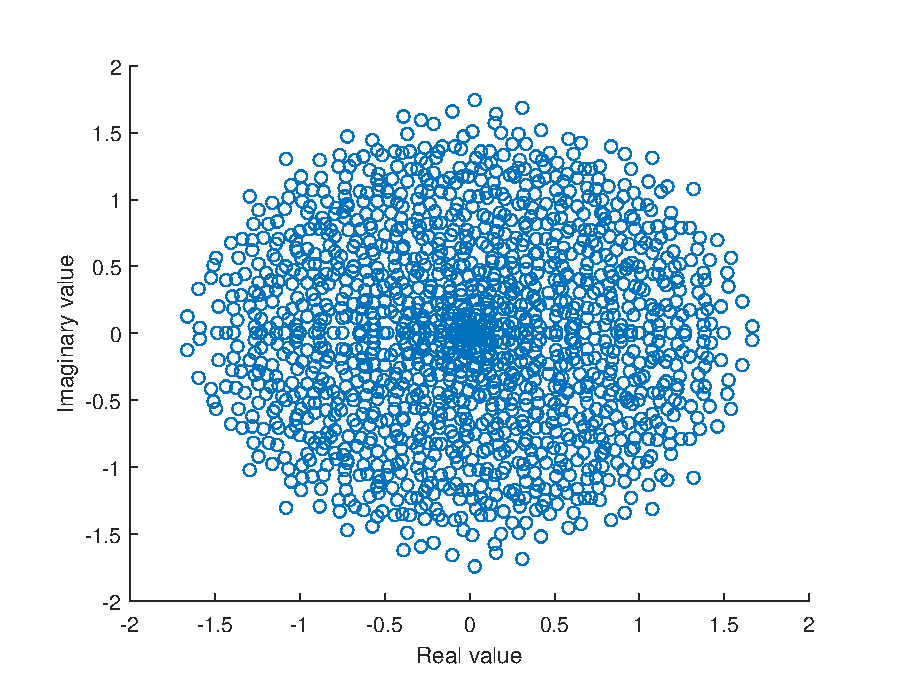
\includegraphics[width=\textwidth]{mat02_spectrum.eps}
				\caption{The spectrum of mat02.}
				\label{fig:mat02spectrum}
			\end{subfigure}
			~ 
			\begin{subfigure}[b]{0.65\textwidth}
				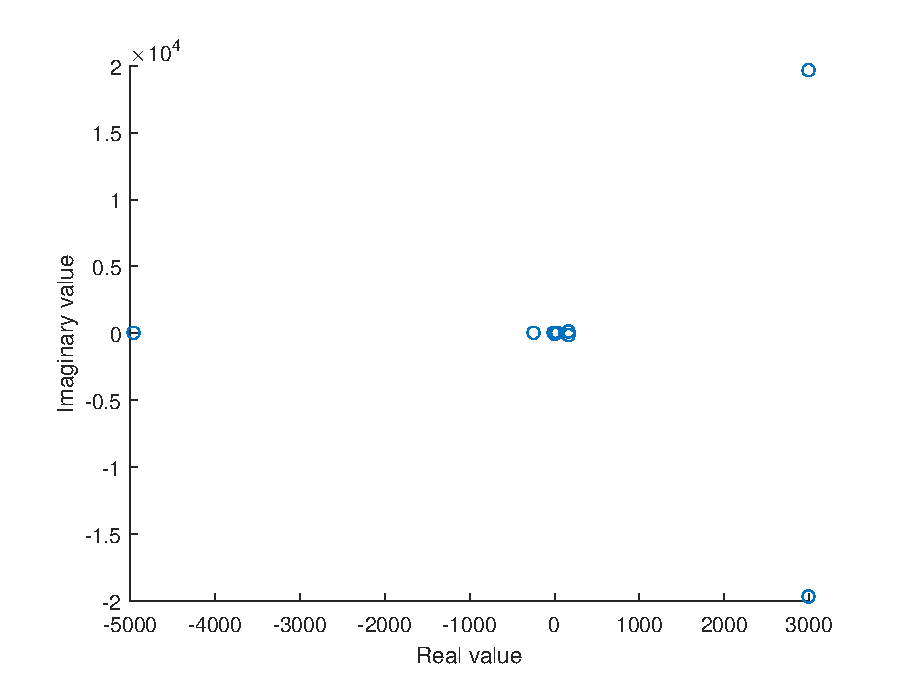
\includegraphics[width=\textwidth]{ARMS34_mat02_spec.eps}
				\caption{The spectrum of the preconditioner multiplied with mat02 in which the preconditioner ARMS is used with value k=3 and ARMS\_levels=4.}
				\label{fig:ARMS34mat02spec}
			\end{subfigure}
		}	
		\caption{Spectra of mat01 with and without a preconditioner.}\label{fig:spectramat02}
	\end{figure}
	
	\begin{figure}
		\centering
		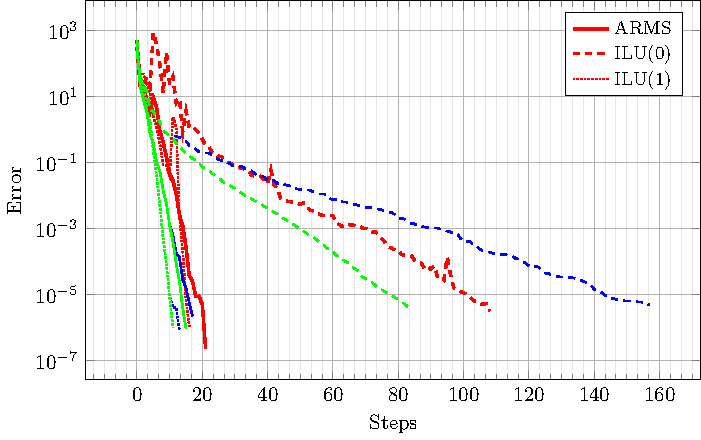
\includegraphics[width=\textwidth]{mat01_error.pdf}
		\caption{The convergence of matrix mat01 with different methods and preconditioners. Red lines are BiCGStab method, blue lines are GMRES(10) and green ones GMRES(100).}
		\label{fig:mat01error} 
	\end{figure}
	
	\begin{figure}
		\centering
		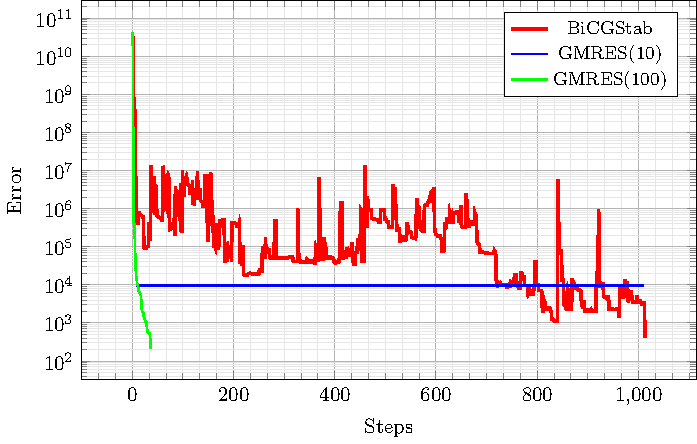
\includegraphics[width=\textwidth]{mat02_error.pdf}
		\caption{The convergence of matrix mat02 with the ARMS preconditioner.}
			\label{fig:mat02error} 
	\end{figure}
		
	\begin{figure}
		\centering
		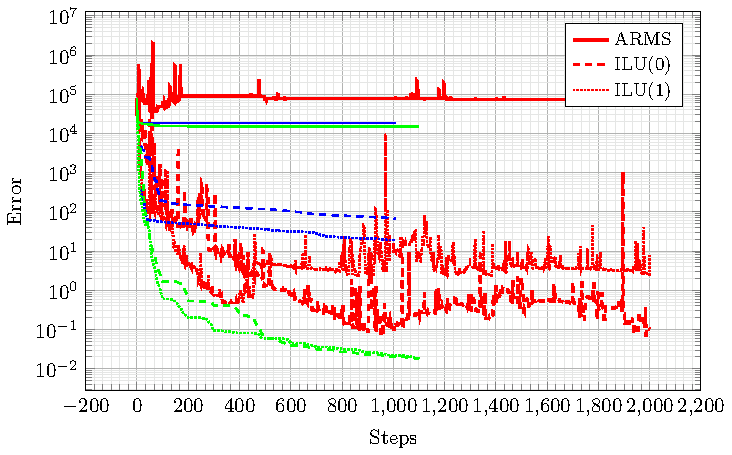
\includegraphics[width=\textwidth]{mat03_error.pdf}
		\caption{The convergence of matrix mat03 with different methods and preconditioners. Red lines are BiCGStab method, blue lines are GMRES(10) and green ones GMRES(100).}
			\label{fig:mat03error} 
	\end{figure}
		
	\begin{figure}
		\centering
		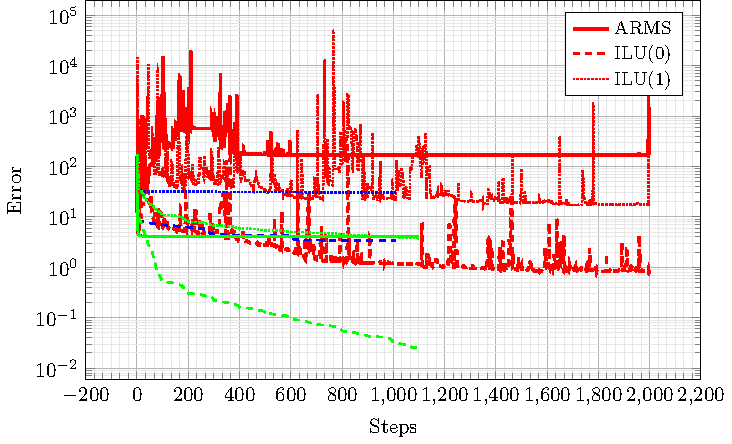
\includegraphics[width=\textwidth]{mat04_error.pdf}
		\caption{The convergence of matrix mat04 with different methods and preconditioners. Red lines are BiCGStab method, blue lines are GMRES(10) and green ones GMRES(100).}
			\label{fig:mat04error} 
	\end{figure}
	
	\begin{figure}
		\centering
		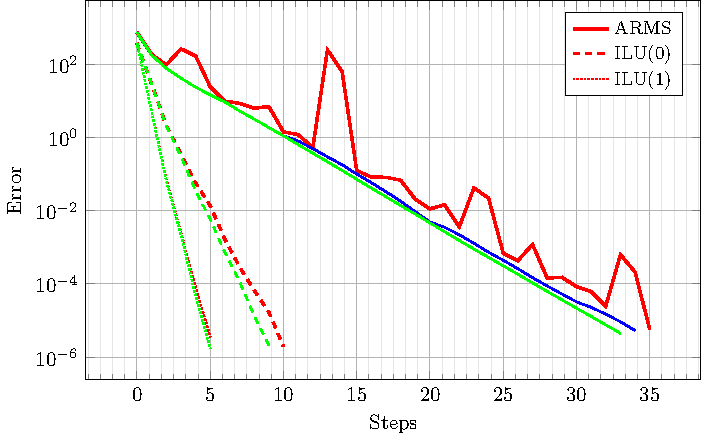
\includegraphics[width=\textwidth]{mat05_error.pdf}
		\caption{The convergence of matrix mat05 with different methods and preconditioners. Red lines are BiCGStab method, blue lines are GMRES(10) and green ones GMRES(100).}
			\label{fig:mat05error} 
	\end{figure}
	
	
	
		 
	
\end{document}
